\documentclass[a4paper]{scrreprt}
\usepackage{xcolor}                % we use grey text here
\usepackage{graphicx}              % figures
\usepackage{listings}              % source code
\usepackage{hyperref}              % navigation
\usepackage{mathptmx}
\usepackage{verbatim}
\usepackage{bold-extra}            % bold keywords in listings
\usepackage[small]{caption}        % better-looking captions
\parindent0mm                      % this looks better in short paragraphs

\hyphenation{An-no-ta-tion-Sketch}

% some colors
\definecolor{arggrey}{gray}{.6}
\definecolor{middlegray}{gray}{.5}
\newcommand{\AnnotationSketch}{\emph{AnnotationSketch}\ }

% listings style
\lstset{
  basicstyle=\scriptsize\ttfamily,
  keywordstyle=\bfseries\ttfamily,
  commentstyle=\color{middlegray}\ttfamily,
  showstringspaces=false,
  flexiblecolumns=false,
  tabsize=2,
  numbers=left,
  numberstyle=\tiny,
  numberblanklines=false,
  stepnumber=1,
  numbersep=10pt,
  xleftmargin=15pt
}

% this is a basic language definition for the listings package
\lstdefinelanguage{Lua}
{
 morecomment = [l]{--},
 morecomment = [s]{--[*[}{]*]--},
 morestring=[b]",
 morestring=[b]',
 sensitive = true,
 morekeywords = {and, break, do, else, elseif, end, for,
    function, if, local, nil, not, or, repeat, return, then,
    until, while}
 morekeywords=[2]{},
}

\title{The \emph{AnnotationSketch} genome annotation drawing library}
\subject{Supplementary Information}
\author{Sascha Steinbiss, Gordon Gremme, Christin Sch\"arfer, Malte Mader\\ and Stefan Kurtz}

\begin{document}

\maketitle

\tableofcontents

\chapter{AnnotationSketch}

\emph{AnnotationSketch} is a versatile and efficient C-based drawing library for GFF3-compatible genomic annotations. It is included in the \emph{GenomeTools} distribution. In addition to the native C interface, bindings to the Lua, Python and Ruby programming languages are provided.

\section{Overview}
\emph{AnnotationSketch} consists of several classes, which take part in
three visualization \emph{phases} (see Fig. \ref{dataflow}).

\begin{figure}[ht]
\centering{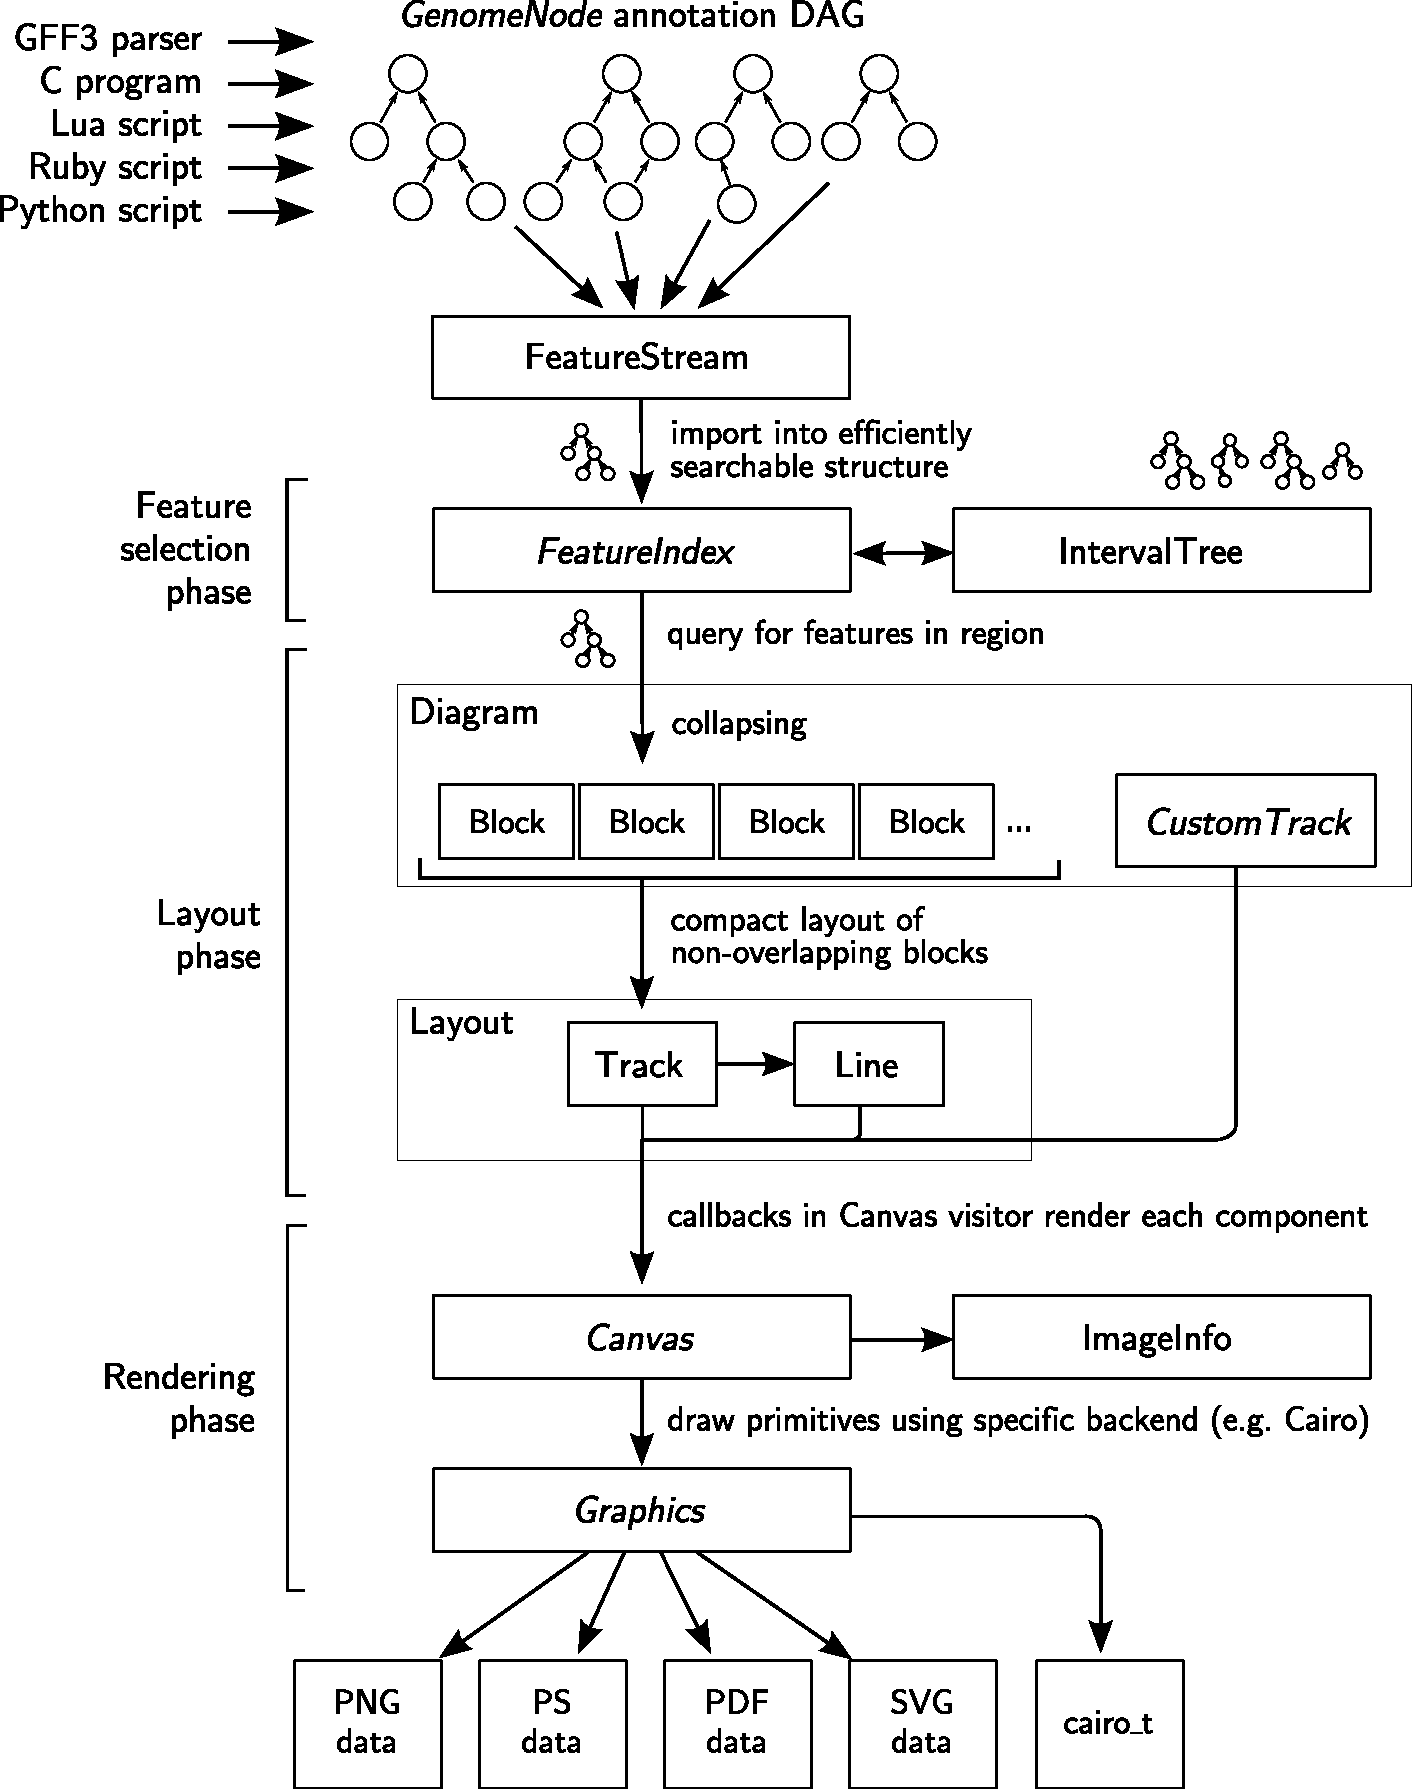
\includegraphics[width=.7\textwidth]{../../www/genometools.org/htdocs/images/dataflow.pdf}}
\caption{Schematic of the data flow through the classes involved in image creation.}
\label{dataflow}
\end{figure}

\subsection{Phase 1: Feature selection}
The GFF3 input data are parsed into a directed acyclic graph (\emph{annotation graph}, see Fig. \ref{gfftree} for an example) whose nodes correspond to single features (i.e. lines from the GFF3 file). Consequently, edges in the graph represent the \emph{part-of} relationships between groups of genomic features according to the Sequence Ontology hierarchy. Note that GFF3 input files \emph{must} be valid according to the GFF3 specification to ensure that they can be read for \AnnotationSketch drawing or any other kind of manipulation using \emph{GenomeTools}. A validating GFF3 parser is available in \emph{GenomeTools} (and can be run using \texttt{gt gff3validator}).

\begin{figure}[ht]
\centering{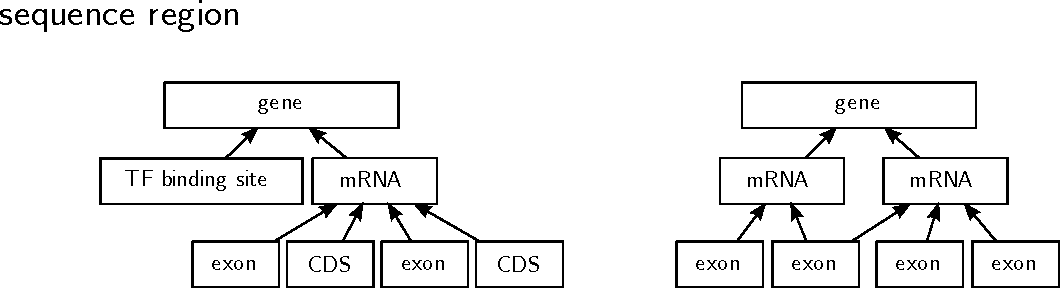
\includegraphics[width=.9\textwidth]{../../www/genometools.org/htdocs/images/gfftree.pdf}}
\caption{Example sequence region containing two genes in an annotation graph depicting the \emph{part-of} relationships between their components.}
\label{gfftree}
\end{figure}
Each top-level node (which is a node without a parent) is then registered into a persistent \emph{FeatureIndex} object. The \emph{FeatureIndex} holds a collection of the top-level nodes of all features in each sequence region in an interval tree data structure that can be efficiently queried for features in a genomic region of interest. All child nodes of the top-level node are then available by the use of traversal functions. Alternatively, annotation graphs can be built by the user by creating each node explicitly and then connecting the nodes in a way such that the relationships are reflected in the graph structure (see examples section for example annotation graph building code).

\subsection{Phase 2: Layout}
The next step consists of processing the features (given via a \emph{FeatureIndex} or a simple array of top level nodes) into a \emph{Diagram} object which represents a single view of the annotations of a genomic region. First, semantic units are formed from the annotation subgraphs. This is done by building \emph{blocks} from connected features by grouping and overlaying them according to several user-defined collapsing options (see ``Collapsing''). By default, a separate \emph{track} is then created for each Sequence Ontology feature type. Alternatively, if more granularity in track assignment is desired, \emph{track selector} functions can be used to create tracks and assign blocks to them based on arbitrary feature characteristics. This is simply done by creating a unique identifier string per track. The \emph{Diagram} object can also be used to hold one or more \emph{custom tracks}, which allow users to develop their own graphical representations as plugins. The \emph{Diagram} is then prepared for image output by calculating a compact \emph{Layout} in which the \emph{Block} objects in a track are distributed into \emph{Line} objects, each containing non-overlapping blocks (see Fig. \ref{diagram}). The overall layout calculated this way tries to keep lines as compact as possible, minimising the amount of vertical space used. How new \emph{Lines} are created depends on the chosen implementation of the \emph{LineBreaker} interface, by default a \emph{Block} is pushed into a new \emph{Line} when either the \emph{Block} or its caption overlaps with another one.

\begin{figure}[ht]
\centering{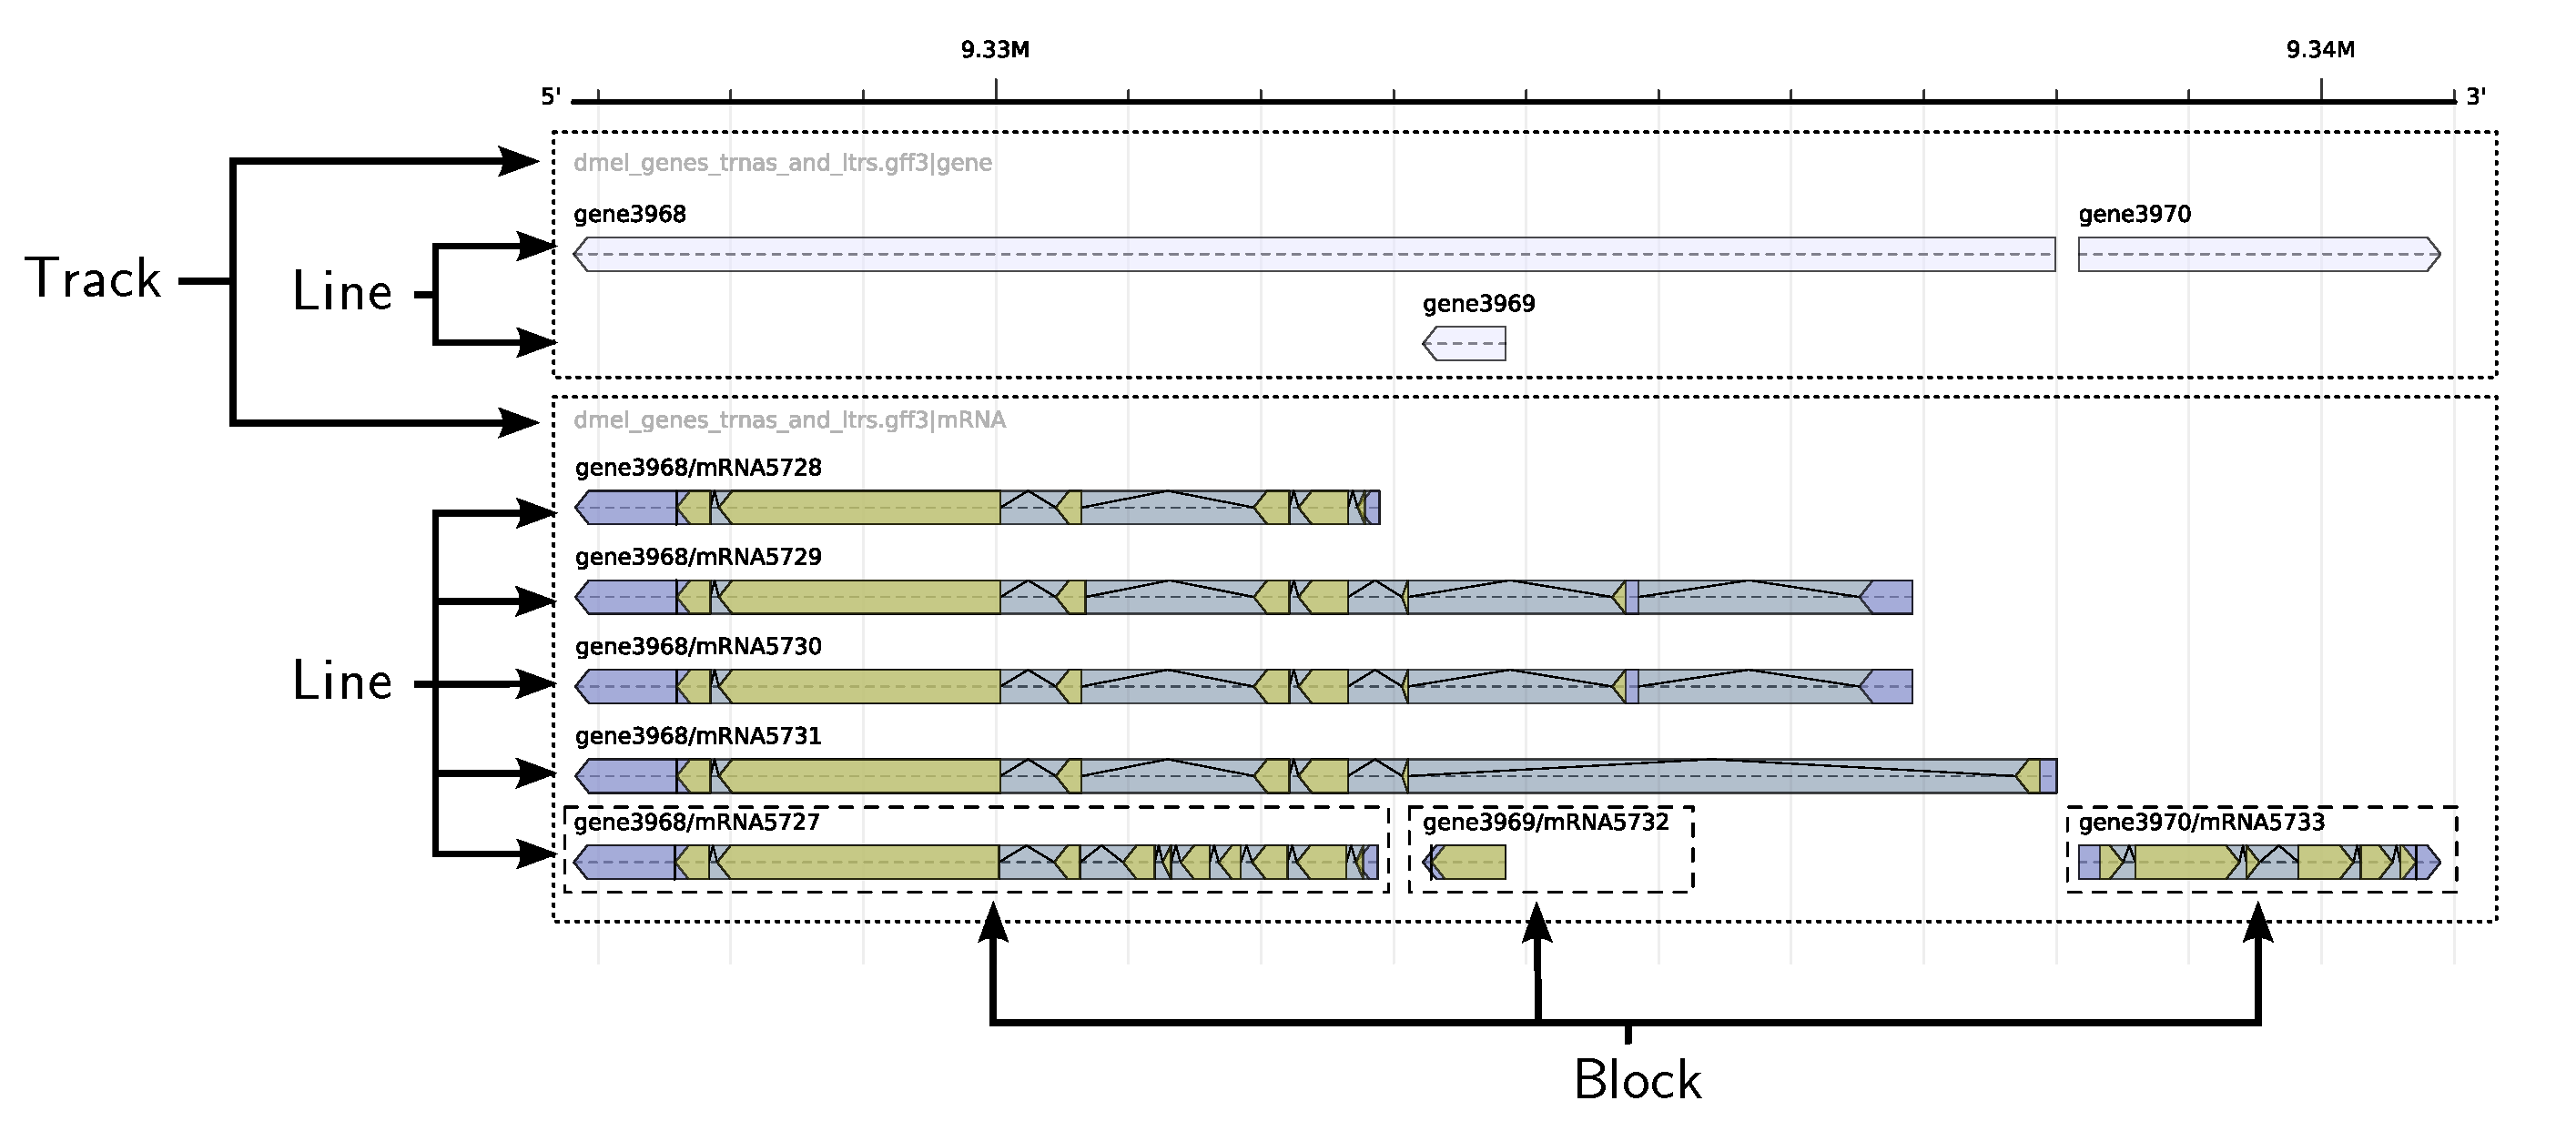
\includegraphics[width=\textwidth]{../../www/genometools.org/htdocs/images/diagram.pdf}}
\caption{The components of the \emph{Layout} class reflect sections of the resulting image.}
\label{diagram}
\end{figure}

\subsection{Phase 3: Rendering}
In the final phase, the \emph{Layout} object is used as a blueprint to create an image of a given type and size, considering user-defined options. The rendering process is invoked by calling the \texttt{sketch()} method of a \emph{Layout} object. All rendering logic is implemented in classes implementing the \emph{Canvas} interface, whose methods are called during traversal of the \emph{Layout} members. It encapsulates the state of a drawing and works independently of the chosen rendering back-end. Instead, rendering backend-dependent subclasses of \emph{Canvas} are closely tied to a specific implementation of the \emph{Graphics} interface, which provides methods to draw a number of primitives to a drawing surface abstraction. It wraps around the respective low-level graphics engine and allows for its easy extension or replacement.
 Currently, there is a \emph{Graphics} implementation for the Cairo 2D graphics library (\emph{GraphicsCairo}) and two \emph{Canvas} subclasses providing access to the image file formats supported by Cairo (\emph{CanvasCairoFile}) and to arbitrary Cairo contexts (\emph{CanvasCairoContext}, which directly accesses a \texttt{cairo\_t}). This class can be used, for example, to directly draw \emph{AnnotationSketch} output in any graphical environment which is supported by Cairo (\url{http://www.cairographics.org/manual/cairo-surfaces.html}).

\subsection{Collapsing}
By default, \emph{Lines} are grouped by the Sequence Ontology type associated with the top-level elements of their \emph{Blocks}, resulting in one track per type.
To obtain a shorter yet concise output, tracks for parent types in the feature graph can be enabled to contain all the features of their child types. The features with the given type are then drawn on top of their parent features (e.g. all \emph{exon} and \emph{intron} features are placed into their parent \emph{mRNA} or \emph{gene} track). This process is called \emph{collapsing}. Collapsing can be enabled by setting the \texttt{collapse\_to\_parent} option for the respective child type to \texttt{true}, e.g. the following options:

\begin{lstlisting}[language=Lua, showstringspaces=false,numbers=none,frame=single]
config = {
  exon = {
    ...,
    collapse_to_parent = true,
    ...,
  },
  intron = {
    ...,
    collapse_to_parent = true,
    ...,
  },
  CDS = {
    ...,
    collapse_to_parent = true,
    ...,
  },
}
\end{lstlisting}
would lead to all features of the \emph{exon}, \emph{intron} and \emph{CDS} types collapsing into the \emph{mRNA} track (see Fig. \ref{collapsetypes} and \ref{cnn_large}).

\begin{figure}
\centering{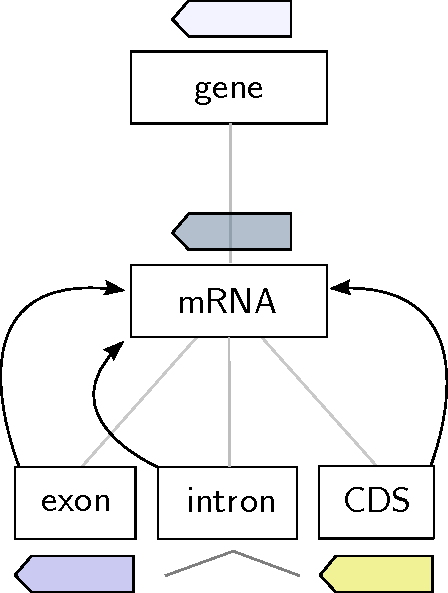
\includegraphics[width=.3\textwidth]{../../www/genometools.org/htdocs/images/collapse_types.pdf}}
\caption{Schematic of the relationships between the \emph{gene}, \emph{mRNA}, \emph{exon}, \emph{intron} and \emph{CDS} types and the colors of their representations in a diagram. The arrows illustrate how the relationships influence the collapsing process if collapsing is enabled for the \emph{exon}, \emph{intron} and \emph{CDS} types. In this example, they will be drawn on top of their parent \emph{mRNA} features.}
\label{collapsetypes}
\end{figure}
\begin{figure}
\centering{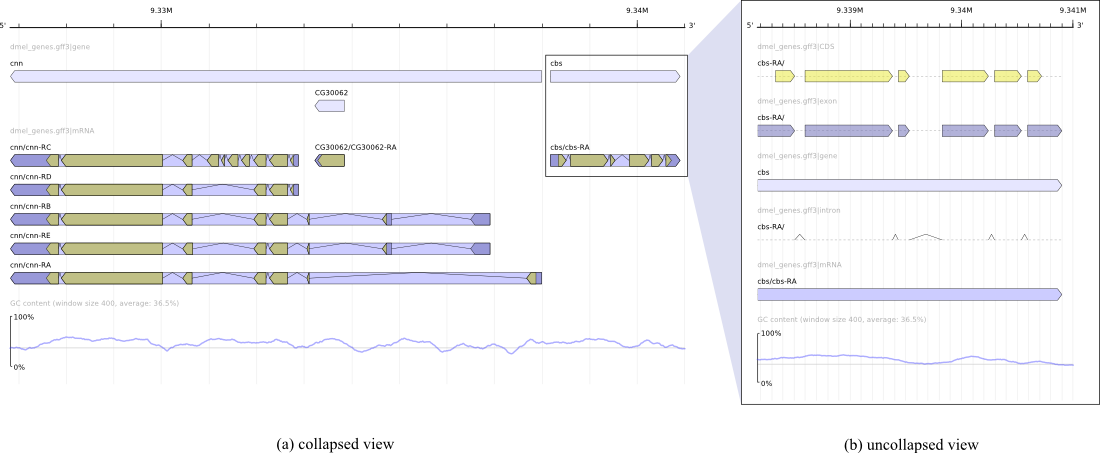
\includegraphics[width=\textwidth]{../../www/genometools.org/htdocs/images/cnn_large}}
\caption{Example image of the \emph{cnn} and \emph{cbs} genes from \emph{Drosophila melanogaster} (Ensembl release 51, positions 9326816--9341000 on chromosome arm 2R) as drawn by \emph{AnnotationSketch}. At the bottom, the calculated GC content of the respective sequence is drawn via a custom track attached to the diagram. (a) shows a collapsed view in which all \emph{exon}, \emph{intron} and \emph{CDS} types are collapsed into their parent type's track. In contrast, (b) shows the \emph{cbs} gene with all collapsing options set to \texttt{false}, resulting in each type being drawn in its own track.}
\label{cnn_large}
\end{figure}


\subsection{Styles}
The Lua scripting language is used to provide
user-defined settings. Settings can be imported from a script that is executed
when loaded, thus eliminating the need for another parser. The Lua configuration
data are made accessible to C via the \emph{Style} class. Configurable options
include assignment of display styles to each feature type, spacer and margin
sizes, and collapsing parameters.

\par Instead of giving direct values, callback Lua functions can be used in some options to generate feature-dependent configuration settings at run-time. During layout and/or rendering, the \emph{GenomeNode} object for the feature to be rendered is passed to the callback function which can then be evaluated and the appropriate type can be returned.
\par For example, setting the following options in the style file (or via the Lua bindings):

\begin{lstlisting}[language=Lua, showstringspaces=false,numbers=left,frame=single]
config = {
  ...,
  mRNA = {
    block_caption      = function(gn)
                           rng = gn:get_range()
                           return string.format("%s/%s (%dbp, %d exons)",
                                 gn:get_attribute("Parent"),
                                 gn:get_attribute("ID"),
                                 rng:get_end() - rng:get_start() + 1,
                                 #(gn:get_exons()))
                         end,
    ...
  },

  exon = {
    -- Color definitions
    fill               = function(gn)
                           if gn:get_score() then
                             aval = gn:get_score()*1.0
                           else
                             aval = 0.0
                           end
                           return {red=1.0, green=0.0, blue=0.0, alpha=aval}
                         end,
    ...
  },
  ...
}

\end{lstlisting}
 will result in a changed rendering (see Fig. \ref{callbacks}). The \texttt{block\_caption} function (line 4) overrides the default block naming scheme, allowing to set custom captions to each block depending on feature properties. Color definitions such as the \texttt{fill} setting (line 17) for a feature's fill color can also be individually styled using callbacks. In this case, the color intensity is shaded by the \emph{exon} feature's score value (e.g. given in a GFF file).

\begin{figure}
\centering{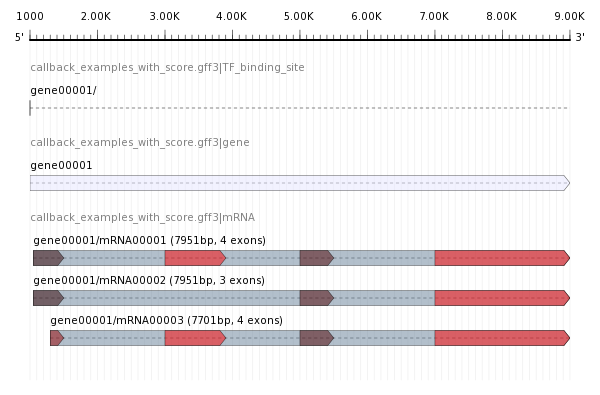
\includegraphics[width=.7\textwidth]{../../www/genometools.org/htdocs/images/callbacks}}
\caption{Example rendering using callback functions to enable custom block captions and score-dependent shading of exon features.}
\label{callbacks}
\end{figure}

\section{The \texttt{gt sketch} tool}

The \emph{GenomeTools} \texttt{gt} executable provides a new tool which uses the \emph{AnnotationSketch} library to create a drawing in PNG, PDF, PostScript or SVG format from GFF3 annotations. The annotations can be given by supplying one or more file names as command line arguments:
\small
\medskip
\begin{verbatim}
$ gt sketch output.png annotation.gff3
$
\end{verbatim}
\normalsize
\medskip
or by receiving GFF3 data via the standard input, here prepared by the \texttt{gt gff3} tool (here called with the \texttt{-addintrons} option to automatically add intron features between exons):
\small
\medskip
\begin{verbatim}
$ gt gff3 -addintrons annotation.gff3 | gt sketch output.png
$
\end{verbatim}
\normalsize
\medskip
The region to create a diagram for can be specified in detail by using the \texttt{-seqid}, \texttt{-start} and \texttt{-end} parameters. For example, if the \emph{D. melanogaster} gene annotation is given in the \texttt{dmel\_annotation.gff3} file, use
\small
\medskip
\begin{verbatim}
$ gt sketch -format pdf -seqid 2R -start 9326816 -end 9332879 output.pdf \
  dmel_annotation.gff3
$
\end{verbatim}
\normalsize
\medskip
to plot a graphical representation of the \emph{cnn} and \emph{cbs} gene region from the \emph{FlyBase} default view in PDF format.
The \texttt{-force} option can be used to force overwriting of an already existing output file. The \texttt{-pipe} option additionally allows passing the GFF3 input through the sketch tool via the standard output, allowing the intermediate visualisation of results in a longer pipeline of connected GFF3 tools. More command line options are available; their documentation can be viewed using the \texttt{-help} option.

If an input file is not plotted due to parsing errors, \emph{GenomeTools} includes a strict GFF3 validator tool to check whether the input file is in valid GFF3 format. Simply run a command like the following:
\small
\medskip
\begin{verbatim}
$ gt gff3validator input_file.gff3
input is valid GFF3
$
\end{verbatim}
\normalsize
\medskip
This validator also allows to check the SO types occurring in a GFF3 file against a given OBO ontology file. This checking can be enabled by specifying the file as an argument to the \texttt{-typecheck} option.

If the PDF, SVG and/or PostScript output format options are not available in the \texttt{gt} binary, the most likely cause is that PDF, SVG and/or PostScript support is disabled in your local \emph{Cairo} headers and thus also not available in your local \emph{Cairo} library. This issue is not directly related to \emph{AnnotationSketch} and can be resolved by recompiling the \emph{Cairo} library with the proper backend support enabled.

\section{Dynamic track assignment}
A special kind of function, called \emph{track selector function}, can be used to customise the \AnnotationSketch output by using arbitrary features of a block to assign blocks to tracks (and implicitly creating new tracks this way).

\subsection{Default: Top level type decides track membership}
By default, for each \emph{Block} in a \emph{Diagram}, its source filename and/or the type attribute of its top level element decides into which track the block is finally inserted during the layout phase. So by default, an annotation graph parsed from the GFF3 input file `example.gff3' with \emph{gene}, \emph{mRNA} and \emph{exon} type nodes will be rendered into two separate tracks (\emph{exon}$\to$\emph{mRNA} collapsing enabled, see Fig.~\ref{tsexample1}):

\begin{itemize}
    \item \texttt{example.gff3|gene}, and
    \item \texttt{example.gff3|mRNA}.
\end{itemize}
We will call the second part (after the ``\texttt{|}'') of these track titles \emph{track identifier strings} in the rest of this document.

\begin{figure}[ht]
\centering{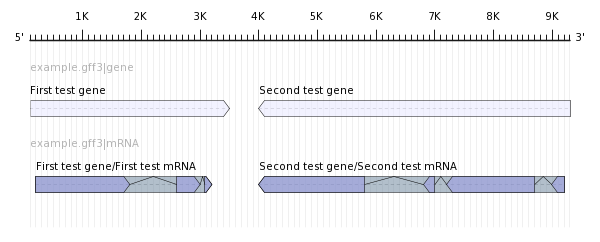
\includegraphics[width=.7\textwidth]{../../www/genometools.org/htdocs/images/example_nocollapse_noselect.png}}
\caption{Default AnnotationSketch output for a simple GFF3 file with simple \emph{exon}$\to$\emph{mRNA} collapsing.}
\label{tsexample1}
\end{figure}

While automatically determining tracks from the types actually present in the input annotations is convenient in many use cases, one could imagine cases in which more control about block handling may be desired. This leads to the question: How can one extract blocks with specific characteristics and assign them to a special track? The answer is simple: By overriding the default track identifier string, new tracks can be created and named on the fly as soon as a block satisfying user-defined rules is encountered.

\subsection{Track selector functions}

These rules take the form of \emph{track selector functions}. Basically, a track selector function is a function which takes a block reference as an argument, and returns an appropriate track identifier string. For example, in Python the default track selector function would look like this:
\begin{lstlisting}[language=Python, showstringspaces=false,numbers=none,frame=single]
def default_track_selector(block):
  return block.get_type()
\end{lstlisting}

This function simply returns a string representation of the type of a block's top level element, creating the tracks just like depicted in Fig. \ref{tsexample1}.

For a very simple example, let's assume that we want to create separate tracks for all mRNAs on the plus strand and for all mRNAs on the minus strand. The idea now is to change the strand identifier for blocks of the \emph{mRNA} type to include the strand as additional information, thus creating different track identifiers for plus and minus strand features. In Python, this track selector function would construct a new string which contains both the type and the strand:

\begin{lstlisting}[language=Python, showstringspaces=false,numbers=none,frame=single]
def strand_track_selector(block):
  if block.get_type() == "mRNA":
    return "%s (%s strand)" % (block.get_type(), block.get_strand())
  else:
    return block.get_type()
\end{lstlisting}

Using this track selector function would produce the desired result of separate tracks for the \emph{mRNA} features for each strand (see Fig. \ref{tsexample2}).

\begin{figure}[ht]
\centering{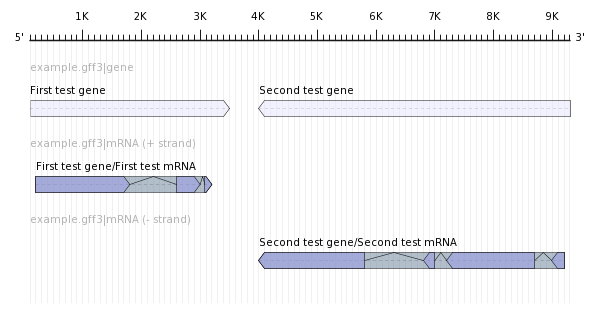
\includegraphics[width=.7\textwidth]{../../www/genometools.org/htdocs/images/example_strandselect.png}}
\caption{AnnotationSketch output with \texttt{strand\_track\_se\-lector()} track selector function. This image now shows separate tracks for plus and minus strand features.}
\label{tsexample2}
\end{figure}

A track selector function can be set for a \emph{Diagram} object using the \texttt{diagram.set\_track\_se\-lec\-tor\_func()} method. In C, its argument is a pointer to a function of the signature
\medskip
\begin{verbatim}
const char* (*GtTrackSelectorFunc)(GtBlock*, void*)
\end{verbatim}
\medskip
where arbitrary data can be passed via the second \texttt{void*} argument. The Python \texttt{set\_track\_se\-lec\-tor\_func()} method directly accepts a Python function as an argument, while the Ruby version takes a Proc object:

\begin{lstlisting}[language=Ruby, showstringspaces=false,numbers=none,frame=single]
...
strand_track_selector = Proc.new { |block, data|
  "#{block.get_type} (#{block.get_strand} strand)"
}
...
diagram.set_track_selector_func(strand_track_selector)
...
\end{lstlisting}

Note that in Python and Ruby, it is also possible to reference data declared outside of the track selector function. For example, this can be used to filter blocks by pulling blocks whose description matches a pattern into a separate track:

\begin{lstlisting}[language=Python, showstringspaces=false,numbers=none,frame=single]
...
interesting_genes = ["First test gene", "another gene"]

def filter_track_selector(block):
  if block.get_caption() in interesting_genes:
    return "interesting genes"
  else:
    return block.get_type()
...
diagram.set_track_selector_func(filter_track_selector)
...
\end{lstlisting}

This code results in the image shown in Fig.~\ref{tsexample3} :

\begin{figure}[ht]
\centering{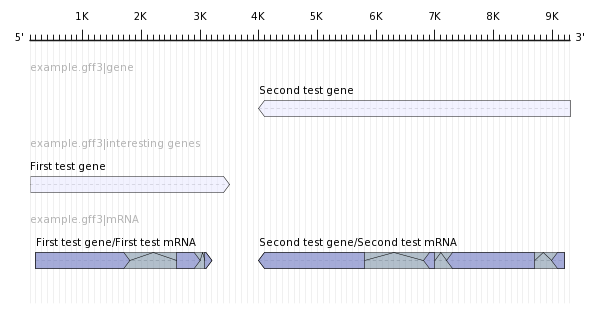
\includegraphics[width=.7\textwidth]{../../www/genometools.org/htdocs/images/example_filterselect.png}}
\caption{\AnnotationSketch output with \texttt{filter\_track\_selector()} track selector function. This image now shows a separate track for features with a specific caption.}
\label{tsexample3}
\end{figure}

\section{Custom tracks}
There are kinds of data which may be interesting to see together with annotation renderings, but that can not be expressed -- or only in a complicated way -- in GFF3 format. It may even be too difficult or counterintuitive to properly represent this data as typical \AnnotationSketch box graphics. For example, this may be sequence data, numerical sequence analysis results, or other kinds of data which does not fit into the simple ‘genomic feature’ scheme. For an example, see Fig. \ref{ctexample1}.

\begin{figure}[ht]
\centering{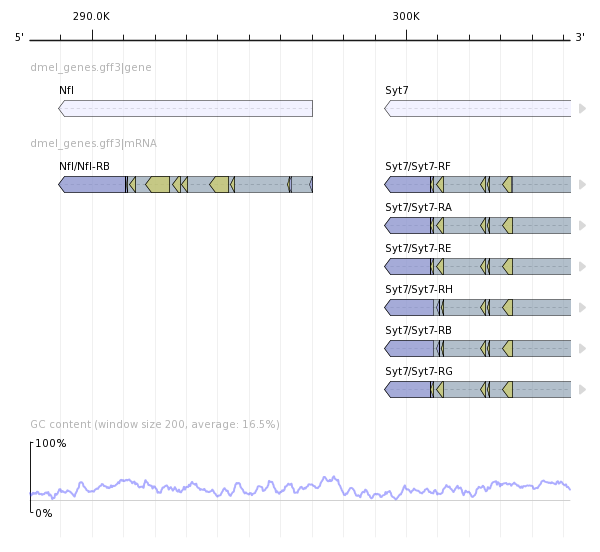
\includegraphics[width=.7\textwidth]{../../www/genometools.org/htdocs/images/example_ct.png}}
\caption{Example \AnnotationSketch output with a custom track at the bottom, displaying the GC content over a window size of 200 bp.}
\label{ctexample1}
\end{figure}

With \emph{custom tracks}, \AnnotationSketch provides a mechanism to use the internal drawing functionality to create user-defined output which can be tailored to fit this kind of data. A custom track looks just like a normal \AnnotationSketch track, but is completely in control of the developer. While native \AnnotationSketch primitives such as boxes can of course be used, the author of a custom track is not restricted to the layout algorithm and can draw anything anywhere (as long as it is provided by the \emph{Graphics} class), taking arbitrary external data into account.

\subsection{Anatomy of a custom track class}

Simply put, custom tracks are classes which are derived from a \emph{CustomTrack} base class and must implement a set of mandatory methods:

\begin{itemize}
    \item \texttt{get\_height()}: Returns the amount of vertical space (in pixels or points) the custom track will occupy in the final image. Must return a numeric value.
    \item \texttt{get\_title()}: Returns a title for the custom track which is displayed at the top of the track. Note that, unlike a track identifier string e.g. produced by a track selector function, the string returned by this function is not prepended by a file name.
    \item \texttt{render(graphics, ypos, range, style, error)}: Performs the actual rendering operations. As parameters, this function receives
       \begin{itemize}
          \item a \emph{Graphics} object to draw on,
          \item the vertical offset \emph{ypos} of the drawing area assigned to the custom track,
          \item the \emph{Range} of the sequence positions for which annotations are currently displayed,
          \item a \emph{Style} object which can be used to obtain style information specific to this custom track, and
          \item an \emph{Error} object which can be used to return an error message if the custom track needs to signal a problem.
        \end{itemize}
\end{itemize}
The \texttt{render()} method must return 0 if drawing was successful, or a negative value if an error occurred.

Optionally, a \texttt{free()} method can be implemented if the subclass needs to clean up any private space allocated by itself. These methods are then called by the rendering code in AnnotationSketch when a Diagram containing a custom track is laid out and rendered. No other constraints apply on such a class besides that these methods are implemented (in the scripting language bindings, the parent classes' constructor must be called once).

\subsection{Writing an example custom track}

Let's suppose we are not satisfied with the display of single base features, such as transposable element insertion sites or SNPs. Instead of a single line denoting the feature location, we would like to have a small triangle pointing at the location. Suppose we also do not have this data in an annotation graph, so we cannot use the built-in rendering functions. It is straightforward to write a small custom track class which does this for us.
This tutorial uses Python code for simplicity, but the general approach is common to all supported languages.

First, we need to define a class inheriting from CustomTrack, call the parent constructor to register the functions and set instance variables for the triangle sidelength and a dictionary containing the feature positions and a description:

\begin{lstlisting}[language=Python, showstringspaces=false,numbers=left,frame=single]
class CustomTrackInsertions(CustomTrack):
  def __init__(self, sidelength, data):
    super(CustomTrackInsertions, self).__init__()
    self.sidelength = sidelength
    self.data = data
\end{lstlisting}

We define the height to be 20 pixels:

\begin{lstlisting}[language=Python, firstnumber=6, showstringspaces=false,numbers=left,frame=single]
  def get_height(self):
    return 20
\end{lstlisting}

As a track title, we set ``Insertion site'':

\begin{lstlisting}[language=Python, firstnumber=8,  showstringspaces=false,numbers=left,frame=single]
  def get_title(self):
    return "Insertion site"
\end{lstlisting}

The rendering code then calculates the triangle coordinates and draws the respective lines:

\begin{lstlisting}[language=Python, firstnumber=10, showstringspaces=false,numbers=left,frame=single]
  def render(self, graphics, ypos, rng, style, error):
    height = (self.sidelength*math.sqrt(3))/2
    margins = graphics.get_xmargins()
    red = Color(1, 0, 0, 0.7)
    for pos, desc in self.data.iteritems():
      drawpos = margins + (float(pos)-rng.start)/(rng.end-rng.start+1)         \
                  * (graphics.get_image_width()-2*margins)
      graphics.draw_line(drawpos-self.sidelength/2, ypos + height,             \
                         drawpos, ypos,                                        \
                         red, 1)
      graphics.draw_line(drawpos, ypos,                                        \
                         drawpos+self.sidelength/2, ypos + height,             \
                         red, 1)
      graphics.draw_line(drawpos-self.sidelength/2, ypos + height,             \
                         drawpos+self.sidelength/2, ypos + height,             \
                         red, 1)
      graphics.draw_text_centered(drawpos, ypos + height + 13, str(desc))
    return 0
\end{lstlisting}

For a Python custom track, that's it! No more code is necessary for this very simple custom track. We can now instantiate this class and attach the instance to a \emph{Diagram} object:

\begin{lstlisting}[language=Python, showstringspaces=false,numbers=none,frame=single]
...
diagram = Diagram(feature_index, seqid, range, style)
...
ctt = CustomTrackInsertions(15, {2000:"foo", 4400:"bar", 8000:"baz"})
diagram.add_custom_track(ctt)
...
\end{lstlisting}

Running layout and drawing functions on this diagram then produces the desired image (see Fig.~\ref{ctexample2}

\begin{figure}[ht]
\centering{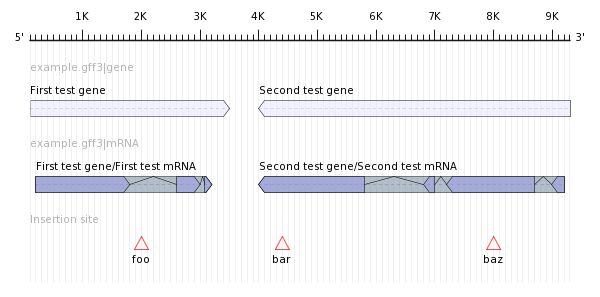
\includegraphics[width=.7\textwidth]{../../www/genometools.org/htdocs/images/example_ct2.png}}
\caption{The example insertion site custom track (at the bottom), displaying three sample data points.}
\label{ctexample2}
\end{figure}

\section{Examples}

This section will show how to use the \emph{AnnotationSketch} library in custom applications. As \emph{AnnotationSketch} is distributed as a part of \emph{GenomeTools}, its code is compiled into the \texttt{lib\-ge\-nome\-tools.so} shared library. Please refer to the INSTALL file inside the \emph{GenomeTools} distribution for installation instructions.

For a general idea about how to use the library, a simple implementation of the GFF3 validator is included in the source package (see \texttt{src/examples/gff3validator.c}) as an example showing how to create \emph{GenomeTools}-based programs. In the same directory, there is also an appropriate \texttt{Makefile} to build and link this application against the installed shared library \texttt{libgenometools.so}.

\subsection{Using \emph{AnnotationSketch} to draw annotations from a file}
The following code examples (in C and Lua) illustrate how to produce an image from a given GFF3 file using \emph{AnnotationSketch}. The result is shown in Fig. \ref{parsed_img}. In essence, these code examples implement something like a simple version of the \texttt{gt sketch} tool from \emph{GenomeTools} without most command-line options. The C-based examples mentioned below are compiled along with the \emph{GenomeTools} library itself and available in the \texttt{bin/examples} directory.

\begin{figure}
\centering{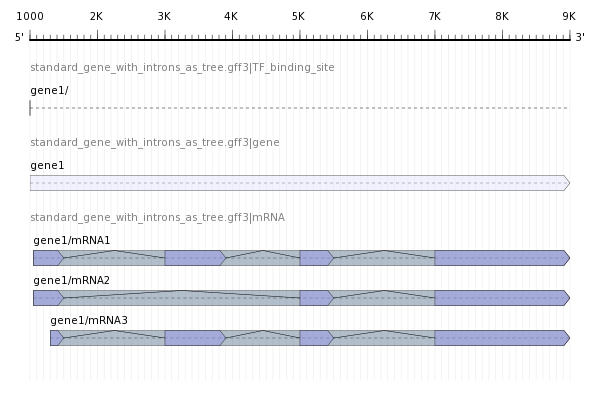
\includegraphics[width=.7\textwidth]{../../www/genometools.org/htdocs/images/parsed}}
\caption{Example rendering of a GFF3 file with default style.}
\label{parsed_img}
\end{figure}

\subsubsection{C code}
(See \texttt{src/examples/sketch\_parsed.c} in the source distribution.)
\lstinputlisting[language=C, breaklines=true, numbers=left, frame=single,]{../../src/examples/sketch_parsed.c}
\subsubsection{Lua code}
(See \texttt{gtscripts/sketch\_parsed.lua} in the source distribution. This example can be run by the command line \texttt{gt gtscripts/sketch\_parsed.lua <style\_file> <PNG\_file> <GFF3\_file>})
\lstinputlisting[language=Lua, breaklines=true, numbers=left, frame=single,]{../../gtscripts/sketch_parsed.lua}
\subsubsection{Ruby code}
(See \texttt{gtruby/sketch\_parsed.rb} in the source distribution.)
\lstinputlisting[language=Ruby, breaklines=true, numbers=left, frame=single,]{../../gtruby/sketch_parsed.rb}
\subsubsection{Python code}
(See \texttt{gtpython/sketch\_parsed.py} in the source distribution.)
\lstinputlisting[language=Python, breaklines=true, numbers=left, frame=single,]{../../gtpython/sketch_parsed.py}

\subsection{Using \emph{AnnotationSketch} to draw user-generated annotations}
The following C code example illustrates how to produce an image from annotation graphs created by user code.
 The result is shown in Fig. \ref{constructed_img}.

\begin{figure}
\centering{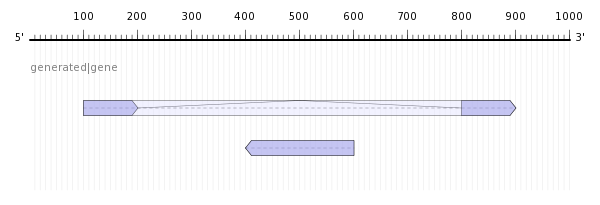
\includegraphics[width=.7\textwidth]{../../www/genometools.org/htdocs/images/constructed}}
\caption{Example rendering of user-generated annotations with default style.}
\label{constructed_img}
\end{figure}

\subsubsection{C code}
(See \texttt{src/examples/sketch\_constructed.c} in the source distribution.)
\lstinputlisting[language=C, breaklines=true, numbers=left, frame=single,]{../../src/examples/sketch_constructed.c}
\subsubsection{Lua code}
(See \texttt{gtscripts/sketch\_constructed.lua} in the source distribution.  This example can be run by the command line \texttt{gt gtscripts/sketch\_constructed.lua <style\_file> <PNG\_file>})
\lstinputlisting[language=Lua, breaklines=true, numbers=left, frame=single,]{../../gtscripts/sketch_constructed.lua}
\subsubsection{Ruby code}
(See \texttt{gtruby/sketch\_constructed.rb} in the source distribution.)
\lstinputlisting[language=Ruby, breaklines=true, numbers=left, frame=single,]{../../gtruby/sketch_constructed.rb}
\subsubsection{Python code}
(See \texttt{gtpython/sketch\_constructed.py} in the source distribution.)
\lstinputlisting[language=Python, breaklines=true, numbers=left, frame=single,]{../../gtpython/sketch_constructed.py}

\input{api_reference}
%\input{gtscript_reference}

\end{document}
